\begin{fullwidth}
\section{An introduction to weak n-categories for formal linguists}

Geometrically, a set is a collection of labelled zero-dimensional points. A category is a collection of one-dimensional labelled arrows upon a set of zero-dimensional points (that satisfy certain additional conditions, such as having identity morphisms and associativity of composition.) Naturally, we might ask what happens when we generalise to more dimensions, asking for two-dimensional somethings going between one-dimensional arrows, and three-dimensional somethings going between two-dimensional somethings, and so on. This is the gist of an $n$-category, where $n$ is a positive integer denoting dimension.\\

There is a fork in the road in generalisation. First, different choices of what n-dimensional somethings could be give different conceptions of $n$-category, because there are multiple mathematically well-founded choices for filling in the blank of \texttt{points, lines, ???}. Simplices, cubical sets, and globular sets are three common options; though the names are fancy, they correspond to triangular, cubical, and circular families of objects indexed by dimension.

\[placeholder\]

Second, there is a distinction between \emph{strict} and \emph{weak} $n$-categories. Just as in regular or $1$-category theory we are interested in objects up to isomorphism rather than equality -- because isomorphic objects in a category are as good as one another -- lifting this philosophy to $n$-categories gives us \emph{weak} $n$-categories. In a strict $k$-category, all of the $j$-dimensional morphisms for $j > k$ are identity-equalities. In a weak $k$-category, all equalities for dimensions $j > k$ are replaced by isomorphisms all the way up: which means that a $k$-equality $\alpha = \beta$ in the strict setting is replaced by a pair of $k+1$-morphisms witnessing the isomorphism of $\alpha$ and $\beta$, and that pair of $k+1$-morphisms has a pair of $k+2$ morphisms witnessing that they are $k+1$-isomorphic, and so on for $k+3$ and all the way up. Unsurprisingly, strict $n$-categories are easy to formalise, and weaks $n$-categories are hard. A conjecture or guiding principle like the Church-Turing thesis holds for weak $n$-categories that they should all be equivalent to one another, whatever equivalence means.\\

Mathematicians, computer scientists, and physicists may have good reasons to work with weak $n$-categories [], but what is the value proposition for formal linguists? A philosophical draw for the formal semanticist is that insofar as semantics is synonymy -- the study of when expressions are equivalent -- weak $n$-categories are an exquisite setting to control and study sameness in terms of meta-equivalences. A practical draw for the formal syntactician is that weak $n$-categories provide a natural setting to model generic rewriting systems, and that is what we will focus on here. In this setting we will introduce weak $n$-categories in the \texttt{homotopy.io} formulation, along the way showing how they provide a common setting to formalise string-rewrite and tree-adjoining grammars, setting the stage for us to specify a circuit-adjoining grammar for text circuits later on. 
\end{fullwidth}

\subsection{String-rewrite systems as 1-object-2-categories}

Say we have an alphabet $\Sigma := \{\textcolor{green}{\alpha}, \textcolor{orange}{\beta}, \textcolor{cyan}{\gamma}\}$. Then the Kleene-star $\Sigma^*$ consists of all strings (including the empty string $\varepsilon$) made up of $\Sigma$, and we consider formal languages on $\Sigma$ to be subsets of $\Sigma^*$. Another way of viewing $\Sigma^*$ is as the free monoid generated by $\Sigma$ under the binary concatenation operation $(\_ \ \cdot \ \_)$ which is associative and unital with unit $\varepsilon$, the empty string. Associativity and unitality are precisely the conditions of composition of morphisms in categories, so we have yet another way to express $\Sigma^*$ as a finitely presented category; we consider a category with a single object $\star$, taking $\varepsilon$ to be the identity morphism $\textbf{1}_\star$ on the single object, and we ask for the category obtained when we consider the closure under composition of three non-identity morphisms $\textcolor{green}{\alpha}, \textcolor{orange}{\beta}, \textcolor{cyan}{\gamma}: \star \rightarrow \star$. In this category, every morphism $\star \rightarrow \star$ corresponds to a string in $\Sigma^*$. We illustrate this example in the margins. A string-rewrite system additionally consists of a finite number of string-transformation rules. Building on our example, we might have a named rule $\textcolor{magenta}{R}: \textcolor{green}{\alpha} \mapsto \textcolor{orange}{\beta} \cdot \textcolor{cyan}{\gamma}$, which we illustrate in Figure \ref{fig:ruleR}.\\

\begin{marginfigure}[10cm]
\centering
\[\tikzfig{ncat/flower1}\]
\caption{The category in question can be visualised as a commutative diagram.}
\end{marginfigure}

\begin{marginfigure}
\centering
\[\resizebox{\textwidth}{!}{\tikzfig{ncat/table1}}\]
\caption{When there are too many generating morphisms, we can instead present the same data as a table of $n$-cells; there is a single 0-cell $\star$, and three non-identity 1-cells corresponding to $\textcolor{green}{\alpha}, \textcolor{orange}{\beta}, \textcolor{cyan}{\gamma}$, each with source and target 0-cells $\star$. Typically identity morphisms can be omitted from tables as they come for free. Observe that composition of identities enforces the behaviour of the empty string, so that for any string $x$, we have $\epsilon \cdot x = x = \epsilon \cdot x$.}
\end{marginfigure}

\begin{marginfigure}
\centering
\[\tikzfig{ncat/cstring1}\]
\caption{For a concrete example, we can depict the string $\textcolor{green}{\alpha} \cdot \textcolor{cyan}{\gamma} \cdot \textcolor{cyan}{\gamma} \cdot \textcolor{orange}{\beta}$ as a morphism in a commuting diagram.}
\end{marginfigure}

\begin{marginfigure}
\centering
\[\tikzfig{ncat/string1}\]
\caption{The string-diagrammatic view, where $\star$ is treated as a wire and morphisms are treated as boxes or dots is an expression of the same data under the Poincar\'{e} dual.}
\end{marginfigure}

\begin{marginfigure}\label{fig:ruleR}
\centering
\[\tikzfig{ncat/poindual}\]
\caption{We can visualise the rule as a commutative diagram where $\textcolor{magenta}{R}$ is a 2-cell between the source and target 1-cells. Just as 1-cells are arrows between 0-cell points in a commuting diagram, a 2-cell can also be conceptualised as a directed surface from a 1-cell to another. Taking the Poincar\'{e} dual of this view gives us a string diagram for the 2-cell $\textcolor{magenta}{R}$.}
\end{marginfigure}

\newthought{We consider rewrites to be equivalent, but not equal.} In a string-rewrite system, rewrites are applied one at a time. This means that even for our simple example, there are two possible rewrites from $\textcolor{green}{\alpha} \cdot \textcolor{green}{\alpha}$ to obtain $\textcolor{orange}{\beta} \cdot \textcolor{cyan}{\gamma} \cdot \textcolor{orange}{\beta} \cdot \textcolor{cyan}{\gamma}$. Here are the two rewrites viewed in two equivalent ways, first on the left informally where strings are nodes in a graph and rewrites are labelled transitions and secondly on the right as two distinct commuting 2-diagrams.

\[\resizebox{0.8\textwidth}{!}{\tikzfig{ncat/2ways}}\]

What should we say about how these two different rewrites relate to each other? Let's say Alice is a formal linguist who is only interested in what strings are reachable from others by rewrites -- this is \emph{de rigeur} when we consider formal languages to be subsets of $\Sigma^*$. She might be happy to declare that these two rewrites are simply equal; categorically this is tantamount to her declaring that any two 2-cells in the 1-object-2-category that share the same source and target are in fact the same, or equivalently, that any $n$-cells for $n \geq 3$ are identities. In fact, what Alice really cares to have is a category where the objects are strings from $\Sigma^*$, and the morphisms are a reachability relation by rewrites; this category is \emph{thin}, in that there is at most one arrow between each pair of objects, which forgets what rewrites are applied.

\[\tikzfig{ncat/thinalice}\]

Let's say Bob is a different sort of formal linguist who wants to model the two rewrites as nonequal but equivalent, with some way to keep track of how different equivalent rewrites relate to one another. Bob might want this for example because he wants to show that head-first rewrite strategies are the same as tail-first, so he wants to keep the observation that the two rewrites are equivalent in that they have the same source and target, while keeping the precise order of rewrites distinct. This order-independence of disjoint or non-interfering rewrites is reflected in the interchange law for monoidal categories, which in the case of our example is depicted as:

\[\tikzfig{ncat/bobfat}\]

In fact, Bob gets to express a new kind of rewrite in the middle: the kind where two non-conflicting rewrites happen \emph{concurrently}. The important aspect of Bob's view over Alice's is that equalities have been replaced by isomorphisms between syntactically inequal rewrites. This demotion of equalities to isomorphisms means that Bob is dealing with a \emph{weak} 1-object-2-category; Bob does have 3-cells that relate different 2-cells with the same source and target, but all of Bob's $n$-cells for $n \geq 3$ are isomorphisms, rather than equalities.

\begin{fullwidth}
\subsection{A context free grammar to generate \texttt{Alice sees Bob quickly run to school}}

We can describe a context-free grammar with the same combinatorial rewriting data that specifies planar string diagrams as we have been illustrating so far. One aspect of rewrite systems we adapt for now is the distinction between terminal and nonterminal symbols; terminal symbols are those after which no further rewrites are possible. We capture this string-diagrammatically by modelling terminal rewrites as 2-cells with target equal to the 1-cell identity of the 0-cell $\star$, which amounts to graphically terminating a wire. The generators subscripted $L$ (for \emph{label} or \emph{leaf}) correspond to terminals of the CFG, and represent a family of generators indexed by a lexicon for the language. The generators subscripted $i$ (for \emph{introducing a type}) correspond to rewrites of the CFG.

\[\scalebox{0.5}{\tikzfig{tree2gate/cfg/cfgsignature}}\]

Consider the sentence \texttt{Alice sees Bob quickly run to school}, which we take to be generated by the following context-free grammar derivation, read from left-to-right. We additionally depict the breakdown of the derivation in terms of rewrites of lower dimension from our signature.

\[\scalebox{0.5}{\tikzfig{tree2gate/cfg/bigcfgbreakdown}}\]

\[\scalebox{0.3}{\tikzfig{tree2gate/workedexample/bigcfg}}\]

\subsection{Tree Adjoining Grammars}

Here is a formal but unenlightening definition of \emph{elementary} tree adjoining grammars which we will convert to diagrams. We will deal with the extensions of links and local constraints to adjoining shortly.

\begin{defn}[\emph{Elementary} Tree Adjoining Grammar: Classic Computer Science style]
*A \textbf{TAG} is a tuple $(\mathcal{N}, \mathcal{N}^\downarrow, \mathcal{N}^*, \Sigma, \mathcal{I}, \mathcal{A})$. These denote, respectively:
\begin{itemize}
	\item{ The \emph{non-terminals}:
		\begin{itemize}
			\item{A set of \emph{non-terminal symbols} $\mathcal{N}$ -- these stand in for grammatical types such as $\texttt{NP}$ and $\texttt{VP}$.}
			\item{A bijection $\downarrow: \mathcal{N} \rightarrow \mathcal{N}^\downarrow$ which acts as $\texttt{X} \mapsto \texttt{X}^\downarrow$. Nonterminals in $\mathcal{N}$ are sent to marked counterparts in $\mathcal{N}^\downarrow$, and the inverse sends marked nonterminals to their unmarked counterparts. These markings are \emph{substitution markers}, which are used to indicate when certain leaf nodes are valid targets for a substitution operation -- discussed later.}
			\item{A bijection $*: \mathcal{N} \rightarrow \mathcal{N}^*$ -- the same idea as above. This time to mark \emph{foot nodes} on auxiliary trees, which is structural information used by the adjoining operation -- discussed later.}
	\end{itemize}
	}
	\item{A set of \emph{terminal symbols} $\Sigma$ -- these stand in for the words of the natural language being modelled.}
	\item{The \emph{elementary trees}:
		\begin{itemize}
			\item{A set of \emph{initial trees} $\mathcal{I}$, which satisfy the following constraints:
			\begin{itemize}
				\item{The interior nodes of an initial tree must be labelled with nonterminals from $\mathcal{N}$}
				\item{The leaf nodes of an initial tree must be labelled from $\Sigma \cup \mathcal{N}^{\downarrow}$}
			\end{itemize}
			}
	\item{A set of \emph{auxiliary trees} $\mathcal{A}$, which satisfy the following constraints:
		\begin{itemize}
			\item{The interior nodes of an auxiliary tree must be labelled with nonterminals from $\mathcal{N}$}
			\item{Exactly one leaf node of an auxiliary tree must be labelled with a foot node $\texttt{X}^{*} \in \mathcal{N}^{*}$; moreover, this labelled foot node must be the marked counterpart of the root node label of the tree.}
			\item{All other leaf nodes of an auxiliary tree are labelled from $\Sigma \cup \mathcal{N}^{\downarrow}$}
		\end{itemize}
		}
	\end{itemize}
	}
\end{itemize}
There are two operations to build what are called \emph{derived trees} from elementary and derived trees. These operations are called \emph{substitution} and \emph{adjoining}.
\begin{itemize}
	\item{\emph{Substitution} replaces a substitution marked leaf node $\texttt{X}^\downarrow$ in a tree $\alpha$ with another tree $\alpha'$ that has $\texttt{X}$ as a root node.}
	\item{\emph{Adjoining} takes auxiliary tree $\beta$ with root and foot nodes $\texttt{X},\texttt{X}^\star$, and a derived tree $\gamma$ at an interior node $\texttt{X}$ of $\gamma$. Removing the $\texttt{X}$ node from $\gamma$ separates it into a parent tree with an $\texttt{X}$-shaped hole for one of its leaves, and possibly multiple child trees with \texttt{X}-shaped holes for roots. The result of adjoining is obtained by identifying the root of $\beta$ with the $\texttt{X}$-context of the parent, and making all the child trees children of $\beta$s foot node $\texttt{X}^\star$.}
\end{itemize}
\end{defn}

The essence of a tree-\emph{adjoining} grammar is as follows: whereas for a CFG one grows the tree by appending branches and leaves at the top of the tree (substitution), in a TAG one can also sprout subtrees from the middle of a branch (adjoining). Now we show that this gloss is more formal than it sounds, by the following steps. First we show that the 2-categorical data of a CFG can be transformed into 3-categorical data -- which we call \emph{Leaf-Ansatz} -- which presents a rewrite system that obtains the same sentences as the CFG, by a bijective correspondence between composition of 2-cells in the CFG and constructed 3-cells in the leaf-ansatz. These 3-cells in the leaf ansatz correspond precisely to the permitted \emph{substitutions} in a TAG. Then we show how to model \emph{adjoining} as 3-cells. Throughout we work with a running example, the CFG grammar introduced earlier.

\begin{construction}[Leaf-Ansatz of a CFG]
Given a signature $\mathfrak{G}$ for a CFG, we construct a new signature $\mathfrak{G}'$ which has the same 0- and 1-cells as $\mathfrak{G}$. See the dashed magenta arrows in the schematic below. For each 1-cell wire type $\texttt{X}$ of $\mathfrak{G}$, we introduce a \emph{leaf-ansatz} 2-cell $\texttt{X}^\downarrow$. For each leaf 2-cell $\texttt{X}_L$ in $\mathfrak{G}$, we introduce a renamed copy $\texttt{X}'_L$ in $\mathfrak{G}'$. Now see the solid magenta arrows in the schematic below. We construct a 3-cell in $\mathfrak{G}'$ for each 2-cell in $\mathfrak{G}$, which has the effect of systematically replacing open output wires in $\mathfrak{G}$ with leaf-ansatzes in $\mathfrak{G}'$.
\[\scalebox{0.5}{\tikzfig{tree2gate/tag/CFGtoTAGpattern}}\]
\end{construction}

\begin{example}
The leaf-ansatz construction just makes formal the following observation: there are multiple equivalent ways of modelling terminal symbols in a rewrite system considered string-diagrammatically. One way (which we have already done) is to treat non-terminals as wires and terminals as effects, so that the presence of an open wire available for composition visually indicates non-terminality. Another (which is the leaf-ansatz construction) treats all symbols in a rewrite system as leaves, where bookkeeping the distinction between (non-)terminals occurs in the signature. So for a sentence like \texttt{Bob drinks}, we have the following derivations that match step for step in the two ways we have considered.
\[\scalebox{0.5}{\tikzfig{tree2gate/tag/leafansatzintuition}}\]
\end{example}

\begin{proposition}[Leaf-ansatzes of CFGs are precisely TAGs with only initial trees and substitution]\label{prop:cfgastag1}
\begin{proof}
By construction. Consider a CFG given by 2-categorical signature $\mathfrak{G}$, with leaf-ansatz signature $\mathfrak{G}'$. The types $\texttt{X}$ of $\mathfrak{G}$ become substitution marked symbols $\texttt{X}^{\downarrow}$ in $\mathfrak{G}'$. The trees $\texttt{X}_i$ in $\mathfrak{G}$ become initial trees $\texttt{X}^0$ in $\mathfrak{G}'$. The 3-cells $\texttt{X}_s$ of $\mathfrak{G}'$ are precisely substitution operations corresponding to appending the 2-cells $\texttt{X}_i$ of $\mathfrak{G}$.
\end{proof}
\end{proposition}

\begin{example}[Leaf-ansatz signature of \texttt{Alice sees Bob quickly run to school} CFG]
\[\scalebox{0.5}{\tikzfig{tree2gate/tag/CFGasTAGsign}}\]
\end{example}

\begin{example}[Adjoining is sprouting subtrees in the middle of branches]
One way we might obtain the sentence \texttt{Bob runs to school} is to start from the simpler sentence \texttt{Bob runs}, and then refine the verb \texttt{runs} into \texttt{runs to school}. This refinement on part of an already completed sentence is not permitted in CFGs, since terminals can no longer be modified. The adjoining operation of TAGs gets around this constraint by permitting rewrites in the middle of trees, as follows:
\[\scalebox{0.5}{\tikzfig{tree2gate/tag/3compareintuition}}\]
\end{example}

\begin{example}[TAG signature of \texttt{Alice sees Bob quickly run to school}]
The highlighted 2-cells are auxiliary trees that replace CFG 2-cells for verbs with sentential complement, adverbs, and adpositions. The highlighted 3-cells are the tree adjoining operations of the auxiliary trees.
\[\scalebox{0.5}{\tikzfig{tree2gate/tag/tagsignature}}\]
\end{example}

The construction yields as a corollary an alternate proof of Theorem [Joshi 6.1.1...]...

\begin{corollary}
For every context-free grammar $\mathfrak{G}$ there exists a tree-adjoining grammar $\mathfrak{G}'$ such that $\mathfrak{G}$ and $\mathfrak{G}'$ are strongly equivalent -- both formalisms generate the same set of strings (weak equivalence) and the same abstract syntactic structures (in this case, trees) behind the strings (strong equivalence).
\begin{proof}
Proposition \ref{prop:cfgastag1} provides one direction of both equivalences. For the other direction, we have to show that each auxiliary tree (a 2-cell) and its adjoining operation (a 3-cell) in $\mathfrak{G}'$ corresponds to a single 2-cell tree of some CFG signature $\mathfrak{G}$, which we demonstrate by construction. See the example above; the highlighted 3-cells of $\mathfrak{G}'$ are obtained systematically from the auxiliary 2-cells as follows: the root and foot nodes $\texttt{X},\texttt{X}^\star$ indicate which wire-type to take as the identity in the left of the 3-cell, and the right of the 3-cell is obtained by replacing all non-$\texttt{X}$ open wires $\texttt{Y}$ with their leaf-ansatzes $\texttt{Y}^\downarrow$. This establishes a correspondence between any 2-cells of $\mathfrak{G}$ considered as auxiliary trees in $\mathfrak{G}'$.
\end{proof}
\end{corollary}

\subsection{Tree adjoining grammars with local constraints}

The usual conception of TAGs includes two extensions to the basic definition presented above. First, there may be \emph{local constraints} on adjoining, which only allows certain trees to be adjoined at certain nodes. Second, TAGs may have links, which are extra edges between nodes obeying a c-command condition. Here we deal with local constraints; dealing with links requires the introduction of braiding.

\begin{defn}[TAG with local constraints: CS-style] [Joshi]
$G = (I,A)$ is a TAG with local constraints if for each node $n$ and each tree $t$, exactly one of the following constraints is specified:
\begin{enumerate}
\item{Selective adjoining (SA): Only a specified subset $\bar{\beta} \subseteq A$ of all auxiliary trees are adjoinable at $n$.}
\item{Null adjoining (NA): No auxiliary tree is adjoinable at the node $n$.}
\item{Obligatory Adjoining (OA): At least one out of all the auxiliary trees adjoinable at $n$ must be adjoined at $n$.}
\end{enumerate}
\end{defn}

The $n$-categorical approach easily accommodates local constraints. For (SA), whereas before we take the source of adjoining rewrites to be identities, we can instead introduce ansatz endomorphisms that are rewritable to the desired subsets. For (NA), we assert that identities have no rewrites (NA). For (OA), we can make a distinction between finished and unfinished derivations, where we require that unfinished derivations are precisely those that still contain an obligatory-rewrite endomorphism.

\begin{example}[Selective and null adjoining diagrammatically]
The below is a reproduction of Example 2.5 of [Joshi] which demonstrates the usage of selective and null adjoining. The notation from [Joshi] is presented first, followed by their corresponding representations in an $n$-categorical signature. The initial tree is presented as a 2-cell where the (SA) rules are rewritable nodes, that serve as sources of rewrites in the 3-cell presentations of the auxiliary trees.
\[\resizebox{\textwidth}{!}{\tikzfig{tree2gate/tag/ex25}}\]
\end{example}

\begin{example}[Obligatory adjoining diagrammatically]
The below is a reproduction of Example 2.11 of [Joshi] which demonstrates the usage of obligatory adjoining, marked orange. The notation from [Joshi] is presented first, followed by their corresponding representations in an $n$-categorical signature. The initial tree is presented as a 2-cell where the (OA) rule is given its own 2-cell, which is the source of rewrites in 3-cell presentations of auxiliary trees. We may capture the obligatory nature of the rewrite by asking that finished derivations contain no instance of the orange 2-cell.
\[\resizebox{\textwidth}{!}{\tikzfig{tree2gate/tag/ex211}}\]
\end{example}

\subsection{Braiding, symmetries, and suspension}

Before we can model TAGs with links, we must introduce the concepts of braiding and symmetries, which we have seen in the diagrammatic setting already as wires twisting past one another. In our current setting of 1-object-3-categories for TAGs, the diagrams we are dealing with are all planar -- i.e. wires may not cross -- but this is a restriction we must overcome when we are dealing with links.\\

First we observe that in a 1-object-2-categorical setting, a morphism from the identity $\varepsilon$ on the base object $\star$ to itself would, in our analogy with string-rewrite systems, be a rewrite from the empty string to itself. For example, a rewrite $R$ may introduce a symbol from the empty string and then delete it. A rewrite $S$ may create a pair of symbols from nothing and then annihilate them.

\[R := \varepsilon \mapsto x \mapsto \varepsilon \quad\quad\quad\quad S := \varepsilon \mapsto a \cdot b \mapsto \varepsilon\]

In our analogy with string rewrite systems, we might like that the following rewrites are equivalent, while respecting that they are not equal.

\begin{enumerate}
\item{Start and finish $R$ and $S$ concurrently, $R$ on the left and $S$ on the right: $\varepsilon = \varepsilon \cdot \varepsilon \mapsto x \cdot a \cdot b \mapsto \varepsilon \cdot \varepsilon = \varepsilon$}
\item{Start $R$ first. Start $S$ on the right concurrently as $R$ finishes: $\varepsilon \mapsto x = x \cdot \epsilon \mapsto \epsilon \cdot a \cdot b = a \cdot b \mapsto \epsilon$}
\item{Start and finish $R$ first, and then start and finish $S$: $\varepsilon \mapsto x \mapsto \varepsilon \mapsto a \cdot b \mapsto \varepsilon$}
\item{Start $S$ first. Start $R$ on the right concurrently as $S$ finishes: $\varepsilon \mapsto a \cdot b = a \cdot b \cdot \varepsilon \mapsto \varepsilon \cdot x = x \mapsto \varepsilon $}
\item{Do $S$ and $R$ concurrently, $S$ on the left and $R$ on the right: $\varepsilon = \varepsilon \cdot \varepsilon \mapsto a \cdot b \cdot x \mapsto \varepsilon \cdot \varepsilon = \varepsilon $}
\end{enumerate}

Diagrammatically, we may represent these rewrites from left to right as follows, representing $x,a,b$ as blue, red, and green wires respectively:

\[\resizebox{\textwidth}{!}{\tikzfig{ncat/xab}}\]

Such rewrites from the empty string to itself are more generally called \emph{scalars} in the monoidal setting, viewed 2-categorically. We may generally represent such scalars as labelled dots. A fact about scalars in a 1-object-2-category called the Eckmann-Hilton argument [] is that dots may circle around one another, and all of those expressions are equivalent up to homotopy. The mechanism that enables this in our setting is that the empty string is equal to copies of itself, which creates the necessary space for manoeuvering; translating into the $n$-categorical setting, expressions are equivalent up to introducing and contracting identities.

\[\resizebox{\textwidth}{!}{\tikzfig{ncat/eckhilt2}}\]

We may view the homotopies that get us from one rewrite to another as 3-cells, which produces a braid in a pair of wires when viewed as a vignette.

\[\resizebox{\textwidth}{!}{\tikzfig{ncat/eckhilt3braid}}\]

Up to processive isotopies [], which are continuous bijective transformations that don't let wires double back on themselves, we can identify two different braidings that are not continuously deformable to one another in the 3-dimensional space of the vignette. We may depict the two braidings as follows, where wires either go over or under one another.

\[\resizebox{\textwidth}{!}{\tikzfig{ncat/braids}}\]

Now we have a setting in which we can consider wires swapping places. However, having two different ways to swap wires presents a complication. While useful for knot-theory, in symmetric monoidal categories we don't want this distinction. Perhaps surprisingly, this distinction is eliminated if we consider swapping dots in the 3D volume rather than the 2D plane. Now we have to extend our analogy to reach 1-object-4-categories. Just as symbols on a 1D string were encoded as 1-cells on the 0-cell identity initially, our braidings are the behaviour of symbols on the 2D plane, encoded as 2-cells on the 1-cell identity of the 0-cell. So, to obtain symbols in a 3D volume, we want 3-cells on the 2-cell identity of the 1-cell identity of the 0-cell. That is a mouthful, so we instead clumsily denote the stacked identity as $\textbf{1}_{\textbf{1}_\star}$. To obtain a dot in a 3-dimensional volume, we consider a rewrite from $\textbf{1}_{\textbf{1}_\star}$ to itself. These dots also enjoy a version of the Eckmann-Hilton argument in 3 dimensions (which holds for all dimensions 2 and higher). We can depict these swaps by movements in a cubic volume where each axis corresponds to a direction of composition. Whereas on the plane the dots have two ways to swap places -- clockwise and counterclockwise rotation -- in the volume they have two new ways to swap places -- clockwise and counterclockwise in the new dimension. Shown below are two ways to swap left-to-right sequentially composed dots by clockwise rotations in the forward-backward and up-down directions of composition:

\[\resizebox{\textwidth}{!}{\tikzfig{ncat/cubes}}\]

Considering these changes of dot positions in 3D as a 4D vignette gives us braidings again. But this time, they are equivalent up to processive isotopy -- in other words, any two ways of swapping the dots in the volume are continuously deformable to one another in the 4-dimensional space of the vignette. The reason is intuitive: a clockwise and counterclockwise braiding along one composition axis can be mutually deformed by making use of the extra available axis of composition. So we have eliminated the differences between the two kinds of braidings.\\

To recap: We follow the convention that object dimensions start at 0. In a 1-object-2-category we obtain planar string diagrams for monoidal categories, which are equivalent up to processive isotopies in an ambient 2-dimensional space. In a 1-object-3-category, we obtain string diagrams for braided monoidal categories that are equivalent up to processive isotopy in an ambient 3-dimensional space -- the page with depth. In a 1-object-4-category, we obtain string diagrams for symmetric monoidal categories, which are equivalent up to processive isotopies in an ambient 4-dimensional space -- while it is difficult to visualise 4-dimensionally, diagrammatically this simplifies dramatically to just allowing wires to cross and only caring about whether input-output connectivity from left to right makes sense. Now observe that for any 1-object-2-category, we can obtain a 1-object-4-category by promoting all 2-cells and higher to sit on top of $\textbf{1}_{\textbf{1}_\star}$, in essence turning dots on a line into dots in a volume; this procedure is called \emph{suspension} []. For example, taking our CFG signature from earlier, suspension promotes 1-cells to 3-cells and 2-cells to 4-cells. The resulting signature gives us the same diagrams, now with the added ability to consider diagrams equivalent up to twisting wires, which models a string-rewrite system with free swapping of symbol order.

\[\scalebox{0.5}{\tikzfig{tree2gate/cfg/cfgsigtwists}}\]

We call the above a 1-object-4-category since there is a single 0-cell, and the first non-identity cell has degree 4. Symmetric monoidal categories are equivalently seen as 1-object-4-categories []. To summarise, by appropriately suspending the signature, we obtain a formal way to power up our diagrams to permit twisting wires, as in symmetric monoidal categories.\\

\begin{remark}[\textbf{THE IMPORTANT TAKEAWAY!}]
Now have a combinatoric way to specify string diagrams that generalises PROPs for symmetric monoidal categories, which in addition permits us to reason with directed diagram rewrites. So we have a trinity of presentations of the same mathematical concept. String diagrams are the \emph{syntax}. Symmetric monoidal categories are the \emph{semantics}. $n$-categories are the \emph{finite combinatoric presentation} of theories and rewrite systems upon them. By analogy, $n$-categories provide a \emph{vocabulary} and \emph{rewrites} for string-diagram \emph{expressions}, which are interpreted with respect to the \emph{context} of a symmetric monoidal category.
\end{remark}

\subsection{TAGs with links}

\begin{defn}[TAGs with links: CS-style]
The following is a reproduction of the discussion on nodes with links from [Joshi]. Linking can be defined for any two nodes in an elementary tree. However, in the linguistic context we will require the following conditions to hold for a link in an elementary tree. If a node $n_1$ is linked to a node $n_2$ then:
\begin{enumerate}
\item{$n_2$ \emph{c-commands} $n_1$, (i.e., $n_2$ is not an ancestor of $n_1$, and there exists a node $m$ which is the immediate parent node of $n_2$, and an ancestor of $n_1$).}
\item{$n_1$ and $n_2$ have the same label.}
\item{$n_1$ is the parent only of a null string, or terminal symbols.}
\end{enumerate}
A \emph{TAG with links} is a TAG in which some of the elementary trees may have links as defined above.
\end{defn}

\begin{example}
The following is a reproduction in \texttt{homotopy.io} of Example 2.4 of [Joshi], illustrating TAGs with links; as a proof assistant for weak $n$-categories, \texttt{homotopy.io} automatically performs tree adjunction after the signature has been properly spelled out. The trees given in Examples 2.4 are:

\[placeholder\]

Which we interpret as expressions comprised of the following signature:

\[placeholder\]

In the process of interpretation, we introduce a link wire-type (in purple), and include directed link generation and elimination morphisms for the $T$ wire-type (in blue). A necessary step in the process of interpretation (which for us involves taking a Poincar\'{e} dual to interpret nodes as wires) is a typing assignment of the tree-branches connected to terminal nodes, which we have opted to read as sharing a $T$-type for minimality, though we could just as well have introduced a separate label-type wire.

\[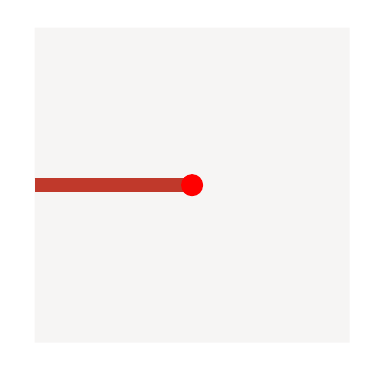
\begin{tikzpicture}
\definecolor{generator-0-0-0-pos}{RGB}{246, 245, 244}
\definecolor{generator-3-5-0-pos}{RGB}{255, 0, 0}
\definecolor{generator-1-4-0-pos}{RGB}{192, 57, 43}
\begin{scope}
% Background surfaces
\fill[generator-0-0-0-pos] (0,-0) -- (0,-4) -- (4,-4) -- (4,-0) -- (0,-0);
% Wire layers
\draw[color=generator-1-4-0-pos, line width=5pt](0,-2) -- (2,-2);
\end{scope}
\fill[generator-3-5-0-pos] (2,-2) circle (0.14) node[anchor=south]{};
\end{tikzpicture}
\]
\[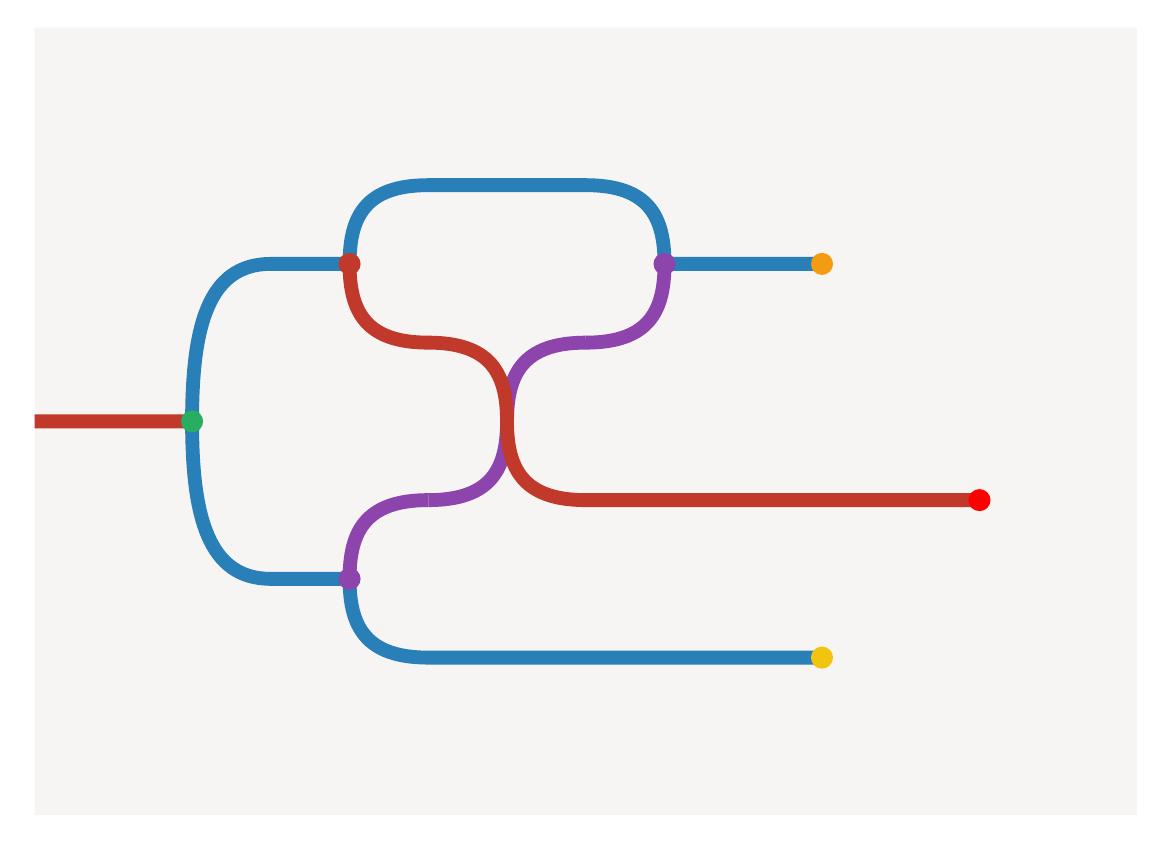
\begin{tikzpicture}
\definecolor{generator-13-5-0-pos}{RGB}{192, 57, 43}
\definecolor{generator-9-4-0-pos}{RGB}{142, 68, 173}
\definecolor{generator-1-4-0-pos}{RGB}{192, 57, 43}
\definecolor{generator-6-5-0-pos}{RGB}{243, 156, 18}
\definecolor{generator-5-5-0-pos}{RGB}{241, 196, 15}
\definecolor{generator-12-5-0-pos}{RGB}{142, 68, 173}
\definecolor{generator-4-5-0-pos}{RGB}{39, 174, 96}
\definecolor{generator-11-5-0-pos}{RGB}{142, 68, 173}
\definecolor{generator-0-0-0-pos}{RGB}{246, 245, 244}
\definecolor{generator-3-5-0-pos}{RGB}{255, 0, 0}
\definecolor{generator-2-4-0-pos}{RGB}{41, 128, 185}
\begin{scope}
% Background surfaces
\fill[generator-0-0-0-pos] (0,-0) -- (0,-10) -- (14,-10) -- (14,-0) -- (0,-0);
% Wire layers
\draw[color=generator-9-4-0-pos, line width=5pt](5,-6) .. controls (5.8,-6) and (6,-5.6) .. (6,-5) .. controls (6,-4.4) and (6.2,-4) .. (7,-4);
\draw[color=generator-1-4-0-pos, line width=5pt](0,-5) -- (2,-5)(4,-3) .. controls (4,-3.6) and (4.2,-4) .. (5,-4) .. controls (5.8,-4) and (6,-4.4) .. (6,-5) .. controls (6,-5.6) and (6.2,-6) .. (7,-6) -- (12,-6);
\draw[color=generator-9-4-0-pos, line width=5pt](4,-7) .. controls (4,-6.4) and (4.2,-6) .. (5,-6)(7,-4) .. controls (7.8,-4) and (8,-3.6) .. (8,-3);
\draw[color=generator-2-4-0-pos, line width=5pt](2,-5) .. controls (2,-3.8) and (2.2,-3) .. (3,-3) -- (4,-3) .. controls (4,-2.4) and (4.2,-2) .. (5,-2) -- (7,-2) .. controls (7.8,-2) and (8,-2.4) .. (8,-3) -- (10,-3)(2,-5) .. controls (2,-6.2) and (2.2,-7) .. (3,-7) -- (4,-7) .. controls (4,-7.6) and (4.2,-8) .. (5,-8) -- (10,-8);
\end{scope}
\fill[generator-4-5-0-pos] (2,-5) circle (0.14);
\fill[generator-13-5-0-pos] (4,-3) circle (0.14);
\fill[generator-12-5-0-pos] (4,-7) circle (0.14);
\fill[generator-11-5-0-pos] (8,-3) circle (0.14);
\fill[generator-6-5-0-pos] (10,-3) circle (0.14);
\fill[generator-5-5-0-pos] (10,-8) circle (0.14);
\fill[generator-3-5-0-pos] (12,-6) circle (0.14);
\end{tikzpicture}
\]
\[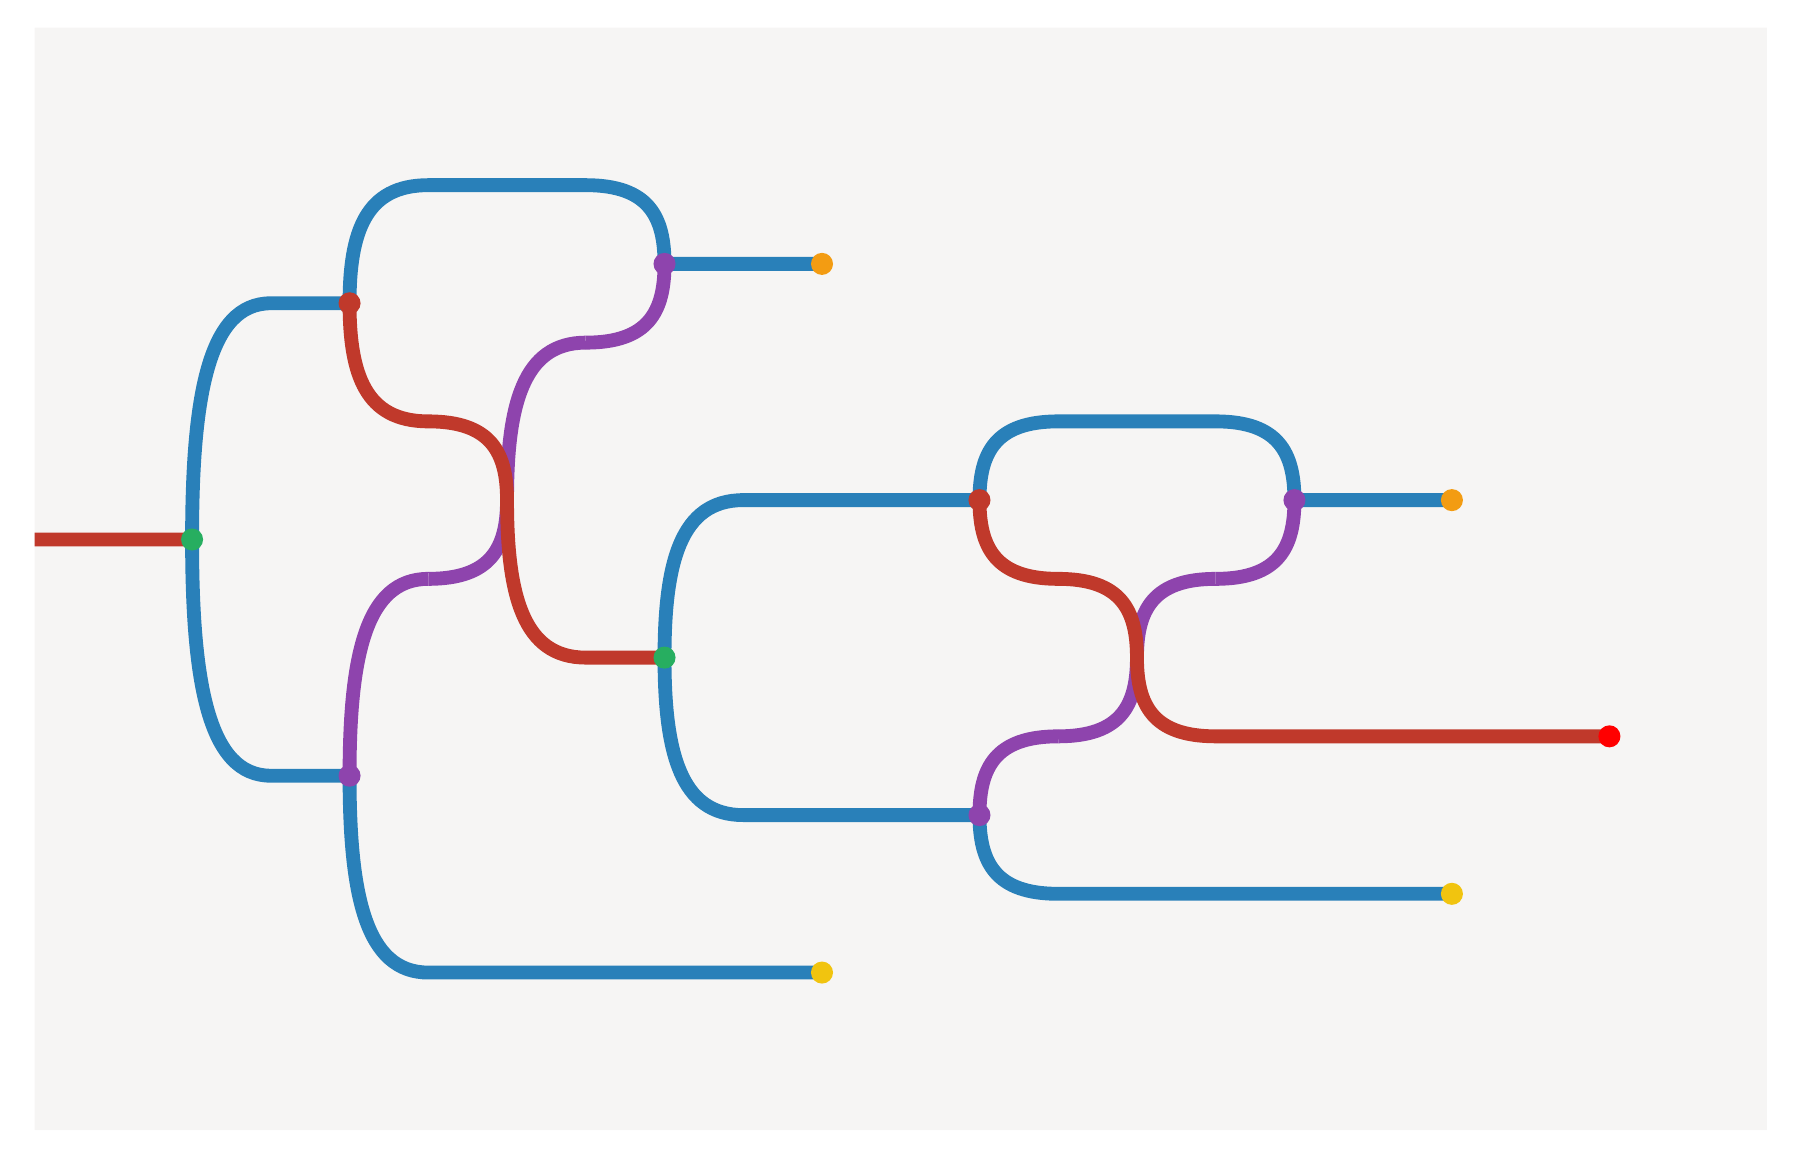
\begin{tikzpicture}
\definecolor{generator-13-5-0-pos}{RGB}{192, 57, 43}
\definecolor{generator-9-4-0-pos}{RGB}{142, 68, 173}
\definecolor{generator-1-4-0-pos}{RGB}{192, 57, 43}
\definecolor{generator-6-5-0-pos}{RGB}{243, 156, 18}
\definecolor{generator-5-5-0-pos}{RGB}{241, 196, 15}
\definecolor{generator-12-5-0-pos}{RGB}{142, 68, 173}
\definecolor{generator-4-5-0-pos}{RGB}{39, 174, 96}
\definecolor{generator-11-5-0-pos}{RGB}{142, 68, 173}
\definecolor{generator-0-0-0-pos}{RGB}{246, 245, 244}
\definecolor{generator-3-5-0-pos}{RGB}{255, 0, 0}
\definecolor{generator-2-4-0-pos}{RGB}{41, 128, 185}
\begin{scope}
% Background surfaces
\fill[generator-0-0-0-pos] (0,-0) -- (0,-14) -- (22,-14) -- (22,-0) -- (0,-0);
% Wire layers
\draw[color=generator-9-4-0-pos, line width=5pt](5,-7) .. controls (5.8,-7) and (6,-6.6) .. (6,-6) .. controls (6,-4.8) and (6.2,-4) .. (7,-4)(13,-9) .. controls (13.8,-9) and (14,-8.6) .. (14,-8) .. controls (14,-7.4) and (14.2,-7) .. (15,-7);
\draw[color=generator-1-4-0-pos, line width=5pt](0,-6.5) -- (2,-6.5)(4,-3.5) .. controls (4,-4.4) and (4.2,-5) .. (5,-5) .. controls (5.8,-5) and (6,-5.4) .. (6,-6) .. controls (6,-7.2) and (6.2,-8) .. (7,-8) -- (8,-8)(12,-6) .. controls (12,-6.6) and (12.2,-7) .. (13,-7) .. controls (13.8,-7) and (14,-7.4) .. (14,-8) .. controls (14,-8.6) and (14.2,-9) .. (15,-9) -- (20,-9);
\draw[color=generator-9-4-0-pos, line width=5pt](4,-9.5) .. controls (4,-8) and (4.2,-7) .. (5,-7)(7,-4) .. controls (7.8,-4) and (8,-3.6) .. (8,-3)(12,-10) .. controls (12,-9.4) and (12.2,-9) .. (13,-9)(15,-7) .. controls (15.8,-7) and (16,-6.6) .. (16,-6);
\draw[color=generator-2-4-0-pos, line width=5pt](2,-6.5) .. controls (2,-4.7) and (2.2,-3.5) .. (3,-3.5) -- (4,-3.5) .. controls (4,-2.6) and (4.2,-2) .. (5,-2) -- (7,-2) .. controls (7.8,-2) and (8,-2.4) .. (8,-3) -- (10,-3)(2,-6.5) .. controls (2,-8.3) and (2.2,-9.5) .. (3,-9.5) -- (4,-9.5) .. controls (4,-11) and (4.2,-12) .. (5,-12) -- (10,-12)(8,-8) .. controls (8,-6.8) and (8.2,-6) .. (9,-6) -- (12,-6) .. controls (12,-5.4) and (12.2,-5) .. (13,-5) -- (15,-5) .. controls (15.8,-5) and (16,-5.4) .. (16,-6) -- (18,-6)(8,-8) .. controls (8,-9.2) and (8.2,-10) .. (9,-10) -- (12,-10) .. controls (12,-10.6) and (12.2,-11) .. (13,-11) -- (18,-11);
\end{scope}
\fill[generator-4-5-0-pos] (2,-6.5) circle (0.14);
\fill[generator-13-5-0-pos] (4,-3.5) circle (0.14);
\fill[generator-12-5-0-pos] (4,-9.5) circle (0.14);
\fill[generator-11-5-0-pos] (8,-3) circle (0.14);
\fill[generator-4-5-0-pos] (8,-8) circle (0.14);
\fill[generator-6-5-0-pos] (10,-3) circle (0.14);
\fill[generator-5-5-0-pos] (10,-12) circle (0.14);
\fill[generator-13-5-0-pos] (12,-6) circle (0.14);
\fill[generator-12-5-0-pos] (12,-10) circle (0.14);
\fill[generator-11-5-0-pos] (16,-6) circle (0.14);
\fill[generator-6-5-0-pos] (18,-6) circle (0.14);
\fill[generator-5-5-0-pos] (18,-11) circle (0.14);
\fill[generator-3-5-0-pos] (20,-9) circle (0.14);
\end{tikzpicture}
\]
\[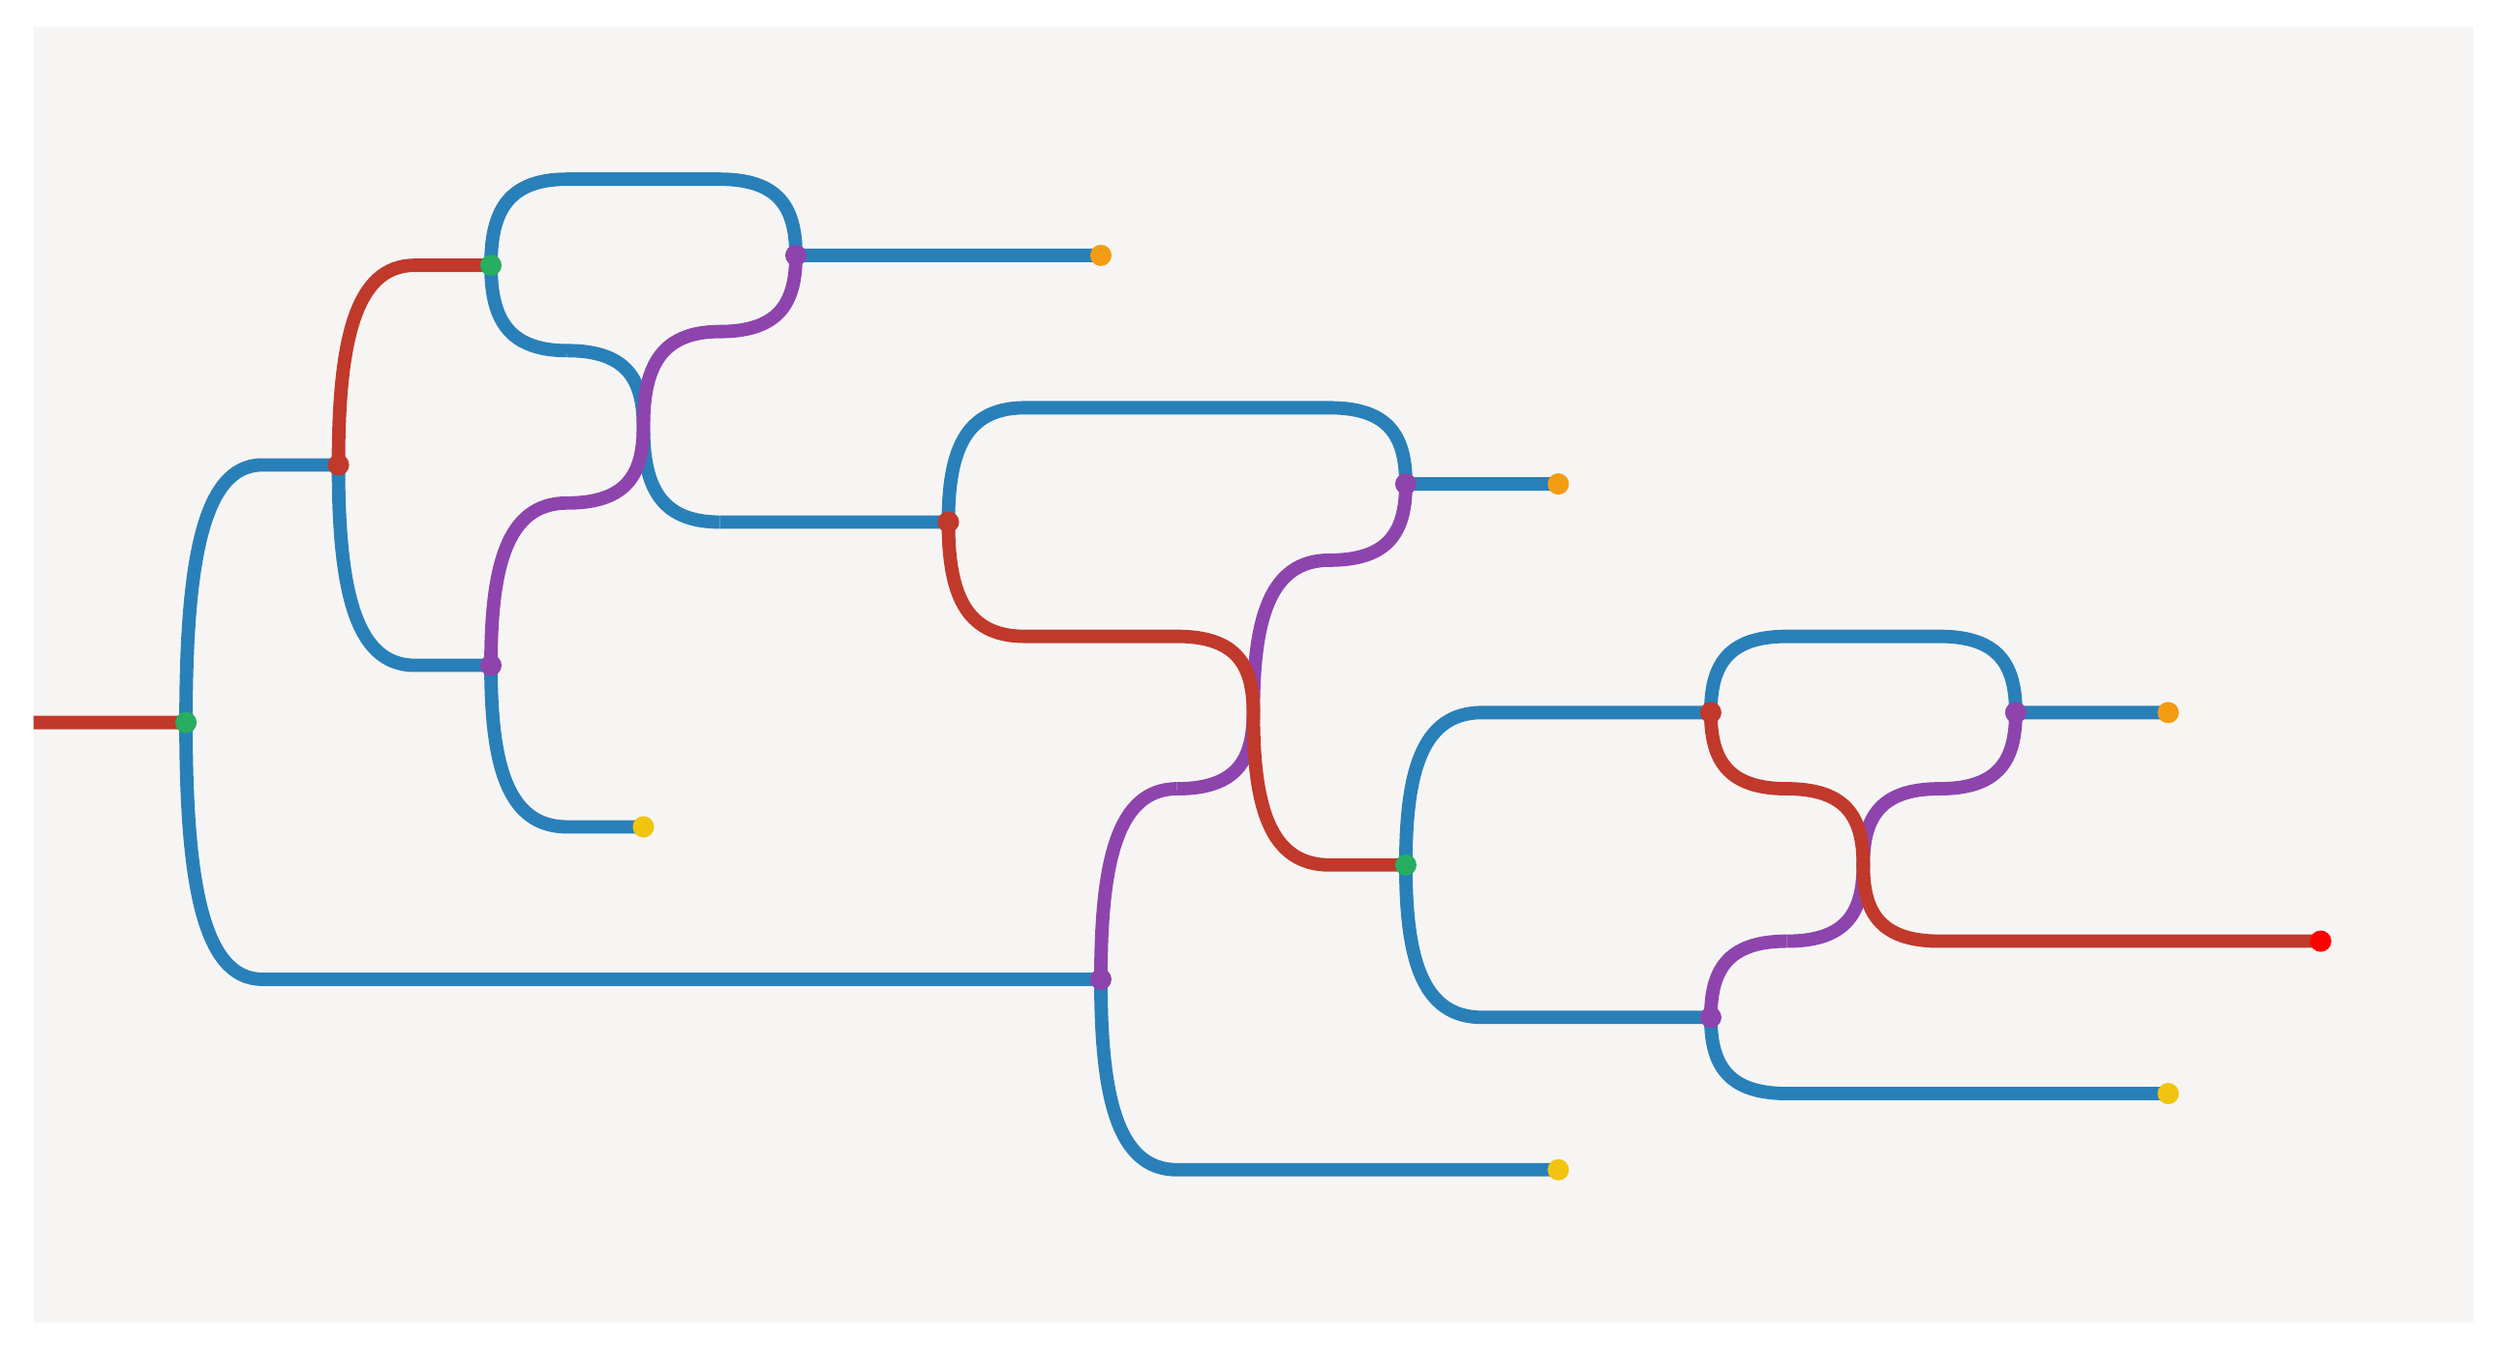
\begin{tikzpicture}
\definecolor{generator-13-5-0-pos}{RGB}{192, 57, 43}
\definecolor{generator-9-4-0-pos}{RGB}{142, 68, 173}
\definecolor{generator-1-4-0-pos}{RGB}{192, 57, 43}
\definecolor{generator-5-5-0-pos}{RGB}{241, 196, 15}
\definecolor{generator-6-5-0-pos}{RGB}{243, 156, 18}
\definecolor{generator-12-5-0-pos}{RGB}{142, 68, 173}
\definecolor{generator-8-5-0-pos}{RGB}{192, 57, 43}
\definecolor{generator-4-5-0-pos}{RGB}{39, 174, 96}
\definecolor{generator-11-5-0-pos}{RGB}{142, 68, 173}
\definecolor{generator-0-0-0-pos}{RGB}{246, 245, 244}
\definecolor{generator-3-5-0-pos}{RGB}{255, 0, 0}
\definecolor{generator-2-4-0-pos}{RGB}{41, 128, 185}
\begin{scope}
% Background surfaces
\fill[generator-0-0-0-pos] (0,-0) -- (0,-17) -- (32,-17) -- (32,-0) -- (0,-0);
% Wire layers
\draw[color=generator-9-4-0-pos, line width=5pt](15,-10) .. controls (15.8,-10) and (16,-9.6) .. (16,-9) .. controls (16,-7.8) and (16.2,-7) .. (17,-7)(23,-12) .. controls (23.8,-12) and (24,-11.6) .. (24,-11) .. controls (24,-10.4) and (24.2,-10) .. (25,-10);
\draw[color=generator-2-4-0-pos, line width=5pt](7,-4.25) .. controls (7.8,-4.25) and (8,-4.65) .. (8,-5.25) .. controls (8,-6) and (8.2,-6.5) .. (9,-6.5);
\draw[color=generator-1-4-0-pos, line width=5pt](0,-9.13) -- (2,-9.13)(4,-5.75) .. controls (4,-4.18) and (4.2,-3.13) .. (5,-3.13) -- (6,-3.13)(12,-6.5) .. controls (12,-7.4) and (12.2,-8) .. (13,-8) -- (15,-8) .. controls (15.8,-8) and (16,-8.4) .. (16,-9) .. controls (16,-10.2) and (16.2,-11) .. (17,-11) -- (18,-11)(22,-9) .. controls (22,-9.6) and (22.2,-10) .. (23,-10) .. controls (23.8,-10) and (24,-10.4) .. (24,-11) .. controls (24,-11.6) and (24.2,-12) .. (25,-12) -- (30,-12);
\draw[color=generator-9-4-0-pos, line width=5pt](6,-8.38) .. controls (6,-7.1) and (6.2,-6.25) .. (7,-6.25) .. controls (7.8,-6.25) and (8,-5.85) .. (8,-5.25) .. controls (8,-4.5) and (8.2,-4) .. (9,-4) .. controls (9.8,-4) and (10,-3.6) .. (10,-3)(14,-12.5) .. controls (14,-11) and (14.2,-10) .. (15,-10)(17,-7) .. controls (17.8,-7) and (18,-6.6) .. (18,-6)(22,-13) .. controls (22,-12.4) and (22.2,-12) .. (23,-12)(25,-10) .. controls (25.8,-10) and (26,-9.6) .. (26,-9);
\draw[color=generator-2-4-0-pos, line width=5pt](2,-9.13) .. controls (2,-7.1) and (2.2,-5.75) .. (3,-5.75) -- (4,-5.75) .. controls (4,-7.33) and (4.2,-8.38) .. (5,-8.38) -- (6,-8.38) .. controls (6,-9.65) and (6.2,-10.5) .. (7,-10.5) -- (8,-10.5)(2,-9.13) .. controls (2,-11.15) and (2.2,-12.5) .. (3,-12.5) -- (14,-12.5) .. controls (14,-14) and (14.2,-15) .. (15,-15) -- (20,-15)(6,-3.13) .. controls (6,-2.45) and (6.2,-2) .. (7,-2) -- (9,-2) .. controls (9.8,-2) and (10,-2.4) .. (10,-3) -- (14,-3)(6,-3.13) .. controls (6,-3.8) and (6.2,-4.25) .. (7,-4.25)(9,-6.5) -- (12,-6.5) .. controls (12,-5.6) and (12.2,-5) .. (13,-5) -- (17,-5) .. controls (17.8,-5) and (18,-5.4) .. (18,-6) -- (20,-6)(18,-11) .. controls (18,-9.8) and (18.2,-9) .. (19,-9) -- (22,-9) .. controls (22,-8.4) and (22.2,-8) .. (23,-8) -- (25,-8) .. controls (25.8,-8) and (26,-8.4) .. (26,-9) -- (28,-9)(18,-11) .. controls (18,-12.2) and (18.2,-13) .. (19,-13) -- (22,-13) .. controls (22,-13.6) and (22.2,-14) .. (23,-14) -- (28,-14);
\end{scope}
\fill[generator-4-5-0-pos] (2,-9.13) circle (0.14);
\fill[generator-8-5-0-pos] (4,-5.75) circle (0.14);
\fill[generator-4-5-0-pos] (6,-3.13) circle (0.14);
\fill[generator-12-5-0-pos] (6,-8.38) circle (0.14);
\fill[generator-5-5-0-pos] (8,-10.5) circle (0.14);
\fill[generator-11-5-0-pos] (10,-3) circle (0.14);
\fill[generator-13-5-0-pos] (12,-6.5) circle (0.14);
\fill[generator-6-5-0-pos] (14,-3) circle (0.14);
\fill[generator-12-5-0-pos] (14,-12.5) circle (0.14);
\fill[generator-11-5-0-pos] (18,-6) circle (0.14);
\fill[generator-4-5-0-pos] (18,-11) circle (0.14);
\fill[generator-6-5-0-pos] (20,-6) circle (0.14);
\fill[generator-5-5-0-pos] (20,-15) circle (0.14);
\fill[generator-13-5-0-pos] (22,-9) circle (0.14);
\fill[generator-12-5-0-pos] (22,-13) circle (0.14);
\fill[generator-11-5-0-pos] (26,-9) circle (0.14);
\fill[generator-6-5-0-pos] (28,-9) circle (0.14);
\fill[generator-5-5-0-pos] (28,-14) circle (0.14);
\fill[generator-3-5-0-pos] (30,-12) circle (0.14);
\end{tikzpicture}
\]

\textbf{N.B.} In practice when using \texttt{homotopy.io} for the symmetric monoidal setting, it is simpler to suspend symmetric monoidal signatures to begin at 4-cells rather than 3-cells. The reason for this is that under- and over-braids still exist in the symmetric monoidal setting, and while sequentially composed braids are homotopically equivalent to the pair of identities, they are not uniquely so, thus these homotopies must be input manually. By beginning at 4-cells (or higher, due to the stabilisation hypothesis []), braid-eliminations are unique up to homotopy and can be performed more easily in the proof assistant.
\end{example}

Now we have enough to spell out full TAGs with local constraints and links as an $n$-categorical signature. To recap briefly, we have seen that we can model the passage from CFGs to TAGs in the $n$-categorical setting, and then how selective and null adjoining rules by specifying endomorphisms on wires as the source of rewrites, and finally that we can model links in the symmetric monoidal setting. Maintaining planarity (which is important for a left-to-right order of terminals for spelling out a language) and modelling obligatory rewrites can be done by requiring that \emph{finished} derivations are precisely those whose only twists are link-wires, and have no sources for obligatory adjoins.

\begin{defn}[Tree Adjoining Grammars with local constraints and links in \texttt{homotopy.io}]

A \emph{Linguistic Tree Adjoining Grammar} is given by the following data:

\[(\mathcal{N}, \mathcal{N}^\downarrow, \mathcal{N}^*, \Sigma, \mathcal{I}, \mathcal{A}, \mathfrak{S} \subseteq \mathcal{P}(\mathcal{A}), \Box, \Diamond, \mathfrak{L} \subseteq \mathcal{N})\]

The initial elements are the same as an elementary tree-adjoining grammar and obey the same constraints. The modifications are:

\begin{itemize}
\item{$\mathcal{I}$ is a nonempty set of \emph{initial} constrained-linked-trees.}
\item{$\mathcal{A}$ is a nonempty set of \emph{auxiliary} constrained-linked-trees.}
\item{$\mathfrak{S}$ is a set of sets of \emph{select} auxiliary trees.}
\item{$\Box, \Diamond$ are fresh symbols. $\Box$ marks \emph{obligatory adjoins}, and $\Diamond$ marks \emph{optional} adjoins.}
\item{$\mathfrak{L}$ is a set permissible \emph{link types} among nonterminals or $\top$.}
\end{itemize}
A \emph{constrained-linked-tree}, or CL-tree, is a pair consisting of:
\begin{itemize}
\item{A tree where each internal node is an element of $\mathcal{N} \times \mathfrak{S} \times \{\Box,\Diamond\} \times \{*, \bar{*}\}$, and each leaf is an element of $\mathcal{N} \times \mathfrak{S} \times \{\Box,\Diamond\} \times \{*, \bar{*}\} \cup \Sigma$. In prose, each label is either a terminal symbol (as a leaf), or otherwise a nonterminal, along with a subset of auxiliary trees that indicates select adjoins (or null-adjoins when the subset is $\varnothing$), a marker indicating whether those adjoins are obligatory or optional, and a marker indicating whether the node is a foot node or not. Observe that there is no need to indicate when a node is a valid target for substitution since that function is subsumed by null adjoining rules.}
\item{
A set of ordered pairs of nodes $(n_1,n_2)$ of the tree such that:
\begin{enumerate}
\item{$n_2$ \emph{c-commands} $n_1$, (i.e., $n_2$ is not an ancestor of $n_1$, and there exists a node $m$ which is the immediate parent node of $n_2$, and an ancestor of $n_1$).}
\item{$n_1$ and $n_2$ share the same type $\mathbf{T} \in \mathcal{N}$ and $\mathbf{T} \in \mathfrak{L}$, or both $n_1,n_2$ are terminals.}
\item{$n_1$ is the parent of terminal symbols, or childless.}
\end{enumerate}
}
\end{itemize}

We spell out how this data becomes an $n$-categorical signature by enumerating cell dimensions:

\begin{enumerate}
\setcounter{enumi}{-1}
\item{A single object $\star$}
\item{None.}
\item{None.}
\item{
	\begin{itemize}
	\item{For each $\mathbf{T} \in \mathcal{N}$, a cell $\mathbf{T}: \mathbf{1}_{\mathbf{1}_\star} \rightarrow \mathbf{1}_{\mathbf{1}_\star}$.}
	\item{$\top: \mathbf{1}_{\mathbf{1}_\star} \rightarrow \mathbf{1}_{\mathbf{1}_\star}$ A wire for terminal symbols.}
	\item{For each $\mathbf{L} \in \mathfrak{L}$, a cell $\mathbf{L} : \mathbf{1}_{\mathbf{1}_\star} \rightarrow \mathbf{1}_{\mathbf{1}_\star}$.}
	\end{itemize}
}
\item{
	We distinguish between \emph{atomic} and \emph{composite} generators at this level. The trees themselves are composites of \emph{atomic} generators. The \emph{atomic} generators are:
	\begin{itemize}
	\item{For each node $n$ that occurs in either $\mathcal{I}$ or $\mathcal{A}$, we populate cells by a case analysis:
	\begin{itemize}
		\item{If $n$ is a terminal $\sigma \in \Sigma$, we create a cell $\sigma: \top \rightarrow \mathbf{1}_{\mathbf{1}_{\mathbf{1}_\star}}$.}
		\item{If $n = (\mathbf{T},\mathbf{S},\dagger,\bar{*})$, we create $\mathbf{S}_\mathbf{T}^\Box: \mathbf{T} \rightarrow \mathbf{T}$ if the node is marked obligatory ($\dagger = \Box$), and a cell $\mathbf{S}_\mathbf{T}^\Diamond: \mathbf{T} \rightarrow \mathbf{T}$ otherwise.}
		\item{If $n = (\mathbf{T},\mathbf{S},\dagger,*)$, it is a foot note, for which we create a cell $\mathbf{S}_\mathbf{T}^\Box: \mathbf{T} \rightarrow \mathbf{1}_{\mathbf{1}_{\mathbf{1}_\star}}$ if the node is marked obligatory ($\dagger = \Box$), and a cell $\mathbf{S}_\mathbf{T}^\Diamond: \mathbf{T} \rightarrow \mathbf{1}_{\mathbf{1}_{\mathbf{1}_\star}}$ otherwise.}
	\end{itemize}
	}
	\item{For each $\mathbf{L} \in \mathfrak{L}$ (which is also a type $\mathbf{T} \in \mathcal{N}$) a pair of cells $\mathbf{T}^\mathbf{L} := \mathbf{T} \rightarrow \mathbf{T} \otimes \mathbf{L}$ and $\mathbf{T}_\mathbf{L} := \mathbf{L} \otimes \mathbf{T} \rightarrow \mathbf{T}$.}
	\item{For each node $p$ of type $\mathbf{T}_p$ in either $\mathcal{I}$ or $\mathcal{A}$ with a nonempty left-to-right list of children $C_p := <c_1,c_2,\cdots c_i, c\dots c_n>$ with types $\mathbf{T}_i$, a branch cell $C_p : \mathbf{T}_p \rightarrow \bigotimes\limits_{i=1}^{n} \mathbf{T}_i$.}
	\end{itemize}
	We represent trees by composite generators, defined recursively. For a given tree $\mathcal{T}$ in either $\mathcal{I}$ or $\mathcal{A}$, we define a composite generator beginning at the root. Where the root node is $p = (\mathbf{T},\mathbf{S},\dagger)$, we begin with the cell $\mathbf{S}_\mathbf{T}^\dagger$. For branches, we compose the branch cell $C_p$ to this cell sequentially. If $p$ has a child $c$ that has a link, we do a case analysis. If that child c-commands the other end of the link we generate the first half of the linking wire by composing $\mathbf{T}^\mathbf{L}$ for the appropriate type $\mathbf{T}$ of the child node. Otherwise the child is c-commanded by a previously generated link, which we braid over and connect using $\mathbf{T}_\mathbf{L}$, again with the appropriate typing for the child. Now we may recurse the procedure for subtrees. If a node has no children, it is a leaf $l = (\mathbf{T},\mathbf{S},\dagger)$ or a terminal symbol. We append a terminal cell $\sigma$ if $l$ is a terminal symbol (thus killing the wire), and otherwise we leave an open $\mathbf{T}$ wire after appending $\mathbf{S}_\mathbf{T}^\dagger$. Altogether this obtains a 3-cell which we denote $\mathcal{T}$, overloading notation; different execution-orders of the above procedure evidently obtain 3-cells equivalent up to homotopy.
}
\item{}
\end{enumerate}

\end{defn}

\end{fullwidth}